% !TEX TS-program = xelatex
% !TEX encoding = UTF-8
\documentclass{aas}
\usepackage{multicol}
\usepackage{subfigure}
\usepackage{amsmath}
\usepackage{amssymb}
\usepackage{amsfonts}
\usepackage{bm}
\usepackage{graphicx}
\usepackage{url}
\usepackage{ccaption}
\usepackage{booktabs} % 做三线表的上下两条粗线用
\usepackage{multirow}

\setcounter{page}{1}

\begin{document}

\cntitle{{\hei\qquad 模拟高机动飞行工况的旋翼建模与升力反馈控制方法}

% TODO: 以下脚注信息(收稿日期/基金/单位/责任编委/作者)请作者补充替换
\thanks{收稿日期\
XXXX-XX-XX
\quad
录用日期\
XXXX-XX-XX}

\thanks{Manuscript received
Month Date, Year;
accepted
Month Date, Year}

\thanks{【待填写基金信息】}

\thanks{Supported by ...}

\thanks{本文责任编委\ XXX}

\thanks{Recommended by Associate Editor XXX}

\thanks{1. 【待填写作者单位与地址】}

\thanks{1. ...}}

\cnauthor{【待填写作者姓名$^{\scriptscriptstyle1}$】}

\cnabstract{多旋翼无人机在高机动飞行过程中,动态倾斜来流作用于桨盘平面,导致旋翼产生的升力出现偏差,本文搭建了能构造此种工况的测试平台,并提出了一种旋翼建模与升力反馈控制方法,旨在能够更快得消除执行器误差,提高升力控制精度.具体来说,采用叶素理论建立考虑桨盘攻角和非均匀来流的旋翼升力机理模型,并结合实验残差构造高保真旋翼模型;基于模型前馈和传感器升力反馈组成旋翼升力闭环控制架构。最后，搭建桨盘攻角与来流速度可调的旋翼测试平台，对单个旋翼构造敏捷机动相关的入流工况；并在旋翼测试台上对所述升力模型和闭环控制架构进行测试。实验结果表明，【待补充定量结果：模型MAE/MAPE、闭环RMSE与峰值误差降低幅度】，从而验证所提方法在高机动工况下提高轴向升力预测与控制精度的有效性。}

\cnkeyword{高机动飞行,旋翼建模,升力反馈控制,高保真模型}

\doi{10.16383/j.aas.20xx.cxxxxxx}

\entitle{Rotor Lift Modeling and Direct Force Feedback Control Method for Oblique Inflow}

% TODO: 英文作者信息请作者补充
\enauthor{SHANG Shu-Lin$^{1}$}

\enabstract{During high-maneuver flight of multirotor UAVs, dynamically tilted inflow acts on the rotor disk plane and causes deviations in the rotor lift. In this paper, a test platform capable of reproducing such operating conditions is constructed, and a rotor modeling and lift feedback control method is proposed to eliminate actuator errors more rapidly and improve lift control accuracy. Specifically, blade element theory is adopted to build a rotor lift mechanism model that considers the disk angle of attack and non-uniform inflow, and experimental residuals are combined to construct a high-fidelity rotor model; a closed-loop rotor lift control architecture is formed based on model feedforward and sensor lift feedback. Finally, a rotor test platform with adjustable disk angle of attack and inflow velocity is built to generate agile-maneuver-related inflow conditions for a single rotor, and the proposed lift model and closed-loop control architecture are tested on this platform. Experimental results show that [quantitative results to be added], which verifies the effectiveness of the proposed method in improving axial lift prediction and control accuracy under high-maneuver conditions.}

\enkeyword{High-maneuver flight, rotor modeling, lift feedback control, high-fidelity model}

\cnaddress{【待填写作者与引用信息】}

\enaddress{【待填写英文作者与引用信息】}

\maketitle

\pagestyle{aasheadings}

%这一章为引言,无需写标题.

近年来，低空经济加速向规模化、常态化运行发展，多旋翼无人机凭借垂直起降、定点悬停和敏捷飞行等特点，已成为物流运输、应急救援、基础设施巡检与复杂环境作业的重要装备[1-3]。随着任务空间由开阔、低速环境拓展至城市近地、山地峡谷和建筑物邻近区域，无人机需要在阵风、尾流、障碍物气动干扰及快速姿态变化条件下保持稳定飞行。此类工况下存在显著旋翼气动效应，通常会影响飞控的PWM控制指令所对应的旋翼升力，进而影响机体姿态和位置控制的稳定性。

现有多旋翼飞控通常根据静态标定得到的升力-控制量映射，将控制分配器输出的期望升力转换为电机控制指令。该映射在近悬停和弱扰动条件下可近似表示为转速或归一化控制量的二次函数，但其参数隐含了特定来流、桨盘姿态和推进系统状态。当无人机快速前飞、转弯或翻转时，旋翼局部来流速度与方向同时变化，桨盘内轴向和盘内速度分量呈现显著非均匀性，继而改变叶素入流角、有效迎角和气动力分布。由此产生的升力偏差首先发生在执行器层，而传统控制架构通常需等待机体姿态或位置误差形成后才能间接修正，难以及时抑制旋翼层面的扰动。

在旋翼层面施加升力反馈能提高多旋翼无人机的控制精度。Gonzalez-Morgado等采用应变片式测力方法，通过检测无人机机臂上产生的形变来间接测量旋翼产生的升力，为提高响应速度，将期望升力通过电机二次模型转换为PWM前馈，并结合PID升力反馈来抑制地面效应和天花板效应。但是这种间接测量方式会引入高频噪声，信噪比低。Jiang等提出了一种直接测量升力的方式，在无人机机臂和旋翼连接处添加了力传感器，并针对旋翼动力系统的非线性，设计了升力反馈线性化控制器；通过单自由度台架实验证明了在风扰环境下能显著提高姿态控制精度。这些工作证明了在存在旋翼气动效应的工况下升力闭环控制的有效性，即提升执行器控制精度能有效抑制气动干扰。

然而，无人机的旋翼动力系统是非线性系统，上述的Jiang等设计了输入输出反馈线性化控制器，并且对动力系统进行复杂的参数辨识，才达到预期控制效果；Gonzalez-Morgado等采用前馈与PID反馈结合的方法，其中前馈项由静态升力-控制量映射得到，实验中地面效应和天花板效应引起的升力误差变化在20\%以内，并且工况相对单一，因此简单前馈加PID即能起到良好效果。

针对复杂来流下的小型螺旋桨气动建模，已有研究形成了实验数据库、机理模型和系统辨识等多条技术路线。Brandt和Selig建立了低雷诺数螺旋桨性能数据库，但数据主要对应轴向来流[4]。Theys等针对0$^{\circ}$-90$^{\circ}$桨盘攻角开展风洞实验并比较叶素动量理论与涡格法[5]；Serrano等进一步评估了非零攻角条件下多种诱导入流模型的预测能力[6]。Simmons利用全攻角风洞数据辨识了包含电机静、动态特性和螺旋桨气动特性的推进系统模型[7]。除风洞外，Itoh和Satoh采用旋转臂测量低前进比下的螺旋桨性能，并对旋转臂诱导速度场进行修正[8]。这些工作为斜来流气动机理与建模提供了重要基础，但实验辨识模型通常依赖特定推进系统和测试包线，直接迁移至其他桨叶与电机组合时仍需重新标定。

在控制层面，研究者通过前飞气动模型、混合数据驱动模型或高保真推进模型改善升力分配与整机控制精度[9-11]。Liu等通过全包线风洞试验辨识推进模型，并将局部雅可比矩阵用于增量非线性动态逆控制，从而提高大机动条件下的控制分配精度[11]。另一类方法直接测量旋翼升力并在电机层闭环。Gonzalez-Morgado等在控制分配器之后引入旋翼力控制器，利用二次模型前馈与力传感器反馈抑制地面效应和天花板效应[12]；相关研究也表明，直接升力感知可缩短执行器扰动被控制系统观测和修正的路径[14,15]。然而，使用静态二次模型作为前馈项时，反馈回路仍需承担动态来流引起的主要模型失配；高保真辨识模型则依赖大量专用试验数据。

为克服上述问题，本文研究：如何在不依赖大规模全包线风洞辨识的前提下，利用桨叶几何和翼型气动信息建立具有可解释性的斜来流推力模型，并将其转化为可在飞控端在线使用的前馈逆映射；同时，如何通过直接推力反馈补偿机理模型残差、动态入流与未建模扰动。为此，本文采用旋转测试台在单旋翼尺度上构造可控的局部来流速度和桨盘攻角。该装置用于复现敏捷机动相关的代表性局部入流条件，而非等比例重现整机飞行轨迹或全部过载环境。

本文的主要工作包括三方面。第一，构建桨盘攻角和转台角速度可调的旋转测试平台，形成面向单旋翼斜来流气动特性与推力控制验证的实验方法。第二，提出由摄影测量桨叶几何、XFOIL翼型极线和非零攻角叶素理论共同约束的轴向推力模型，并在实验校核基础上形成控制导向的简化模型及逆映射。第三，设计模型前馈与直接推力反馈相结合的旋翼推力内环，使机理模型负责提供主要控制量，力反馈负责补偿残差和扰动。全文结构如下：第1节建立旋翼运动状态与斜来流升力机理模型；第2节分析传统控制架构的局限性并给出升力闭环控制架构；第3节介绍实验系统并给出升力模型精度与闭环控制效果的验证结果；第4节总结全文。

\onecolumn\begin{multicols}{2}%这一行用于第一页末尾

\section{旋翼运动状态建模}
\label{sec:rotor_state}

% ============================================================
% 《旋翼运动状态建模》一节  —— 《自动化学报》中文体例
% 依赖宏包：amsmath, amssymb, bm, booktabs（如模板已加载可删去）
% 说明：式号、图号、表号请按正文实际情况调整 \label / \ref
% ============================================================

\subsection{坐标系与符号约定}
\label{subsec:frame}

简化的四旋翼无人机模型如图1所示. 定义机体坐标系
$\mathcal{B}=\{O_b;\bm{x}_b,\bm{y}_b,\bm{z}_b\}$ 为前--右--下坐标系, 原点位于机体质心;
定义惯性坐标系 $\mathcal{I}=\{O_i;\bm{x}_i,\bm{y}_i,\bm{z}_i\}$ 为北--东--地坐标系.
记 $\bm{R}=\bm{R}(\bm{q})\in SO(3)$ 为由 $\mathcal{B}$ 至 $\mathcal{I}$ 的旋转矩阵,
无人机的运动状态由位置 $\bm{p}\in\mathbb{R}^3$、速度 $\bm{v}\in\mathbb{R}^3$、
姿态四元数 $\bm{q}$ 与机体角速度 $\bm{\omega}=[\omega_x,\ \omega_y,\ \omega_z]^{\mathrm{T}}$ 描述, 满足

\begin{equation}
\dot{\bm{p}}=\bm{v},\qquad
\dot{\bm{q}}=\frac{1}{2}\,\bm{q}\otimes
\begin{bmatrix}0\\ \bm{\omega}\end{bmatrix}
\label{eq:body_kinematics}
\end{equation}

设第 $i$ 个旋翼($i=1,2,3,4$)的桨毂中心在机体系下的安装位置为常矢量
$\bm{r}_i\in\mathbb{R}^3$, 桨盘法向单位矢量取为升力正方向, 对于共面等桨距布局有
$\bm{n}_i=[0,\ 0,\ -1]^{\mathrm{T}}$; 若存在安装倾角, 则 $\bm{n}_i$ 为相应的常值单位矢量.
以 $\sigma_i=\pm 1$ 表示旋翼转向, $\sigma_i=+1$ 表示旋翼角速度沿 $+\bm{n}_i$ 方向;
以 $\Omega_i>0$ 表示旋翼转速, $\psi_i$ 表示桨叶方位角(在桨盘平面内自 $\bm{x}_b$ 轴量起).
环境风速在惯性系下记为 $\bm{v}_w$.

\begin{center}
\vbox{
% \centerline{\includegraphics[width=8cm]{Image/fig1.pdf}}
\centerline{【图1：待插入图片】}
\vskip2mm
{\small 图1\quad 四旋翼模型与机体/惯性坐标系定义
\\
Fig.\,1\quad Quadrotor model and definition of body/inertial frames}}
\end{center}

\subsection{桨毂的刚体运动学}
\label{subsec:hub_kinematics}

由于旋翼与机体固连, 在机体系下有 $\dot{\bm{r}}_i\equiv\bm{0}$, 故第 $i$ 个旋翼桨毂
在惯性系下的位置、速度与加速度分别为

\begin{align}
\bm{p}_i&=\bm{p}+\bm{R}\,\bm{r}_i \label{eq:hub_p}\\[2pt]
\bm{v}_i&=\bm{v}+\bm{R}\left(\bm{\omega}\times\bm{r}_i\right) \label{eq:hub_v}\\[2pt]
\bm{a}_i&=\bm{a}+\bm{R}\left[\dot{\bm{\omega}}\times\bm{r}_i
+\bm{\omega}\times\left(\bm{\omega}\times\bm{r}_i\right)\right] \label{eq:hub_a}
\end{align}

式~(\ref{eq:hub_a}) 右端第二项中, $\dot{\bm{\omega}}\times\bm{r}_i$ 为角加速度引起的切向分量,
$\bm{\omega}\times(\bm{\omega}\times\bm{r}_i)$ 为角速度引起的向心分量. 二者共同构成旋翼
所承受的附加过载, 其等效载荷因数为

\begin{equation}
n_i=\frac{\left\|\bm{a}_i-\bm{g}\right\|}{g}
\label{eq:load_factor}
\end{equation}

式~(\ref{eq:load_factor}) 给出了旋转测试台工况设计的依据: 当悬臂长度为 $L$、
臂转速为 $\Omega_r$ 时, 台架为旋翼提供的向心加速度为 $\Omega_r^2 L$,
与式~(\ref{eq:hub_a}) 中机动飞行产生的向心项在形式上一致,
从而可在地面复现高机动工况下的等效过载.

\subsection{桨毂处相对来流的分解}
\label{subsec:inflow}

计入环境风后, 桨毂中心相对于空气的速度在机体系下表示为

\begin{equation}
\bm{u}_i=\bm{R}^{\mathrm{T}}\left(\bm{v}-\bm{v}_w\right)+\bm{\omega}\times\bm{r}_i
\label{eq:u_hub}
\end{equation}

将 $\bm{u}_i$ 沿桨盘法向与桨盘平面内分解, 得到轴向来流速度与面内(侧向)来流速度

\begin{equation}
V_{a,i}=\bm{u}_i^{\mathrm{T}}\bm{n}_i,\qquad
\bm{u}_{\parallel,i}=\left(\bm{I}_3-\bm{n}_i\bm{n}_i^{\mathrm{T}}\right)\bm{u}_i,\qquad
V_{\parallel,i}=\left\|\bm{u}_{\parallel,i}\right\|
\label{eq:decompose}
\end{equation}

其中 $V_{a,i}$ 以爬升方向为正. 相应地, 来流倾角(即来流方向与桨盘平面的夹角)与来流方位角定义为

\begin{equation}
\alpha_i=\arctan\frac{V_{a,i}}{V_{\parallel,i}},\qquad
\psi_{w,i}=\operatorname{atan2}\!\left(u_{i,y},\ u_{i,x}\right)
\label{eq:alpha_psiw}
\end{equation}

设桨半径为 $R_p$, 定义前进比与轴向入流比

\begin{equation}
\mu_i=\frac{V_{\parallel,i}}{\Omega_i R_p},\qquad
\lambda_{c,i}=\frac{V_{a,i}}{\Omega_i R_p}
\label{eq:mu_lambda}
\end{equation}

诱导入流比 $\lambda_{\mathrm{ind},i}$ 由 Glauert 诱导速度模型隐式确定, 尾迹偏斜角为 $\chi_i$:

\begin{equation}
\lambda_{\mathrm{ind},i}=\frac{C_T}{2\sqrt{\mu_i^2+\left(\lambda_{c,i}+\lambda_{\mathrm{ind},i}\right)^2}},
\qquad
\chi_i=\arctan\frac{\mu_i}{\lambda_{c,i}+\lambda_{\mathrm{ind},i}}
\label{eq:glauert}
\end{equation}

式~(\ref{eq:mu_lambda}) 与式~(\ref{eq:alpha_psiw}) 所定义的 $(\mu_i,\ \alpha_i)$
即为旋翼所处的倾斜来流工况点, 也是后文旋转测试台工况编排的自变量.

\subsection{旋翼的转动状态}
\label{subsec:rotation}

第 $i$ 个旋翼相对惯性系的绝对角速度为机体角速度与自转角速度之和

\begin{equation}
\bm{\omega}_i=\bm{\omega}+\sigma_i\Omega_i\bm{n}_i
\label{eq:omega_rotor}
\end{equation}

将式~(\ref{eq:omega_rotor}) 向桨盘法向投影, 得桨叶相对空间的有效转速

\begin{equation}
\Omega_{e,i}=\Omega_i-\sigma_i\,\bm{\omega}^{\mathrm{T}}\bm{n}_i
\label{eq:omega_eff}
\end{equation}

即偏航角速度会使桨叶相对空气的实际转速偏离测量转速. 而机体角速度的面内分量

\begin{equation}
\bm{\omega}_{\parallel}=\left(\bm{I}_3-\bm{n}_i\bm{n}_i^{\mathrm{T}}\right)\bm{\omega}
\label{eq:omega_par}
\end{equation}

不改变转速, 但会在桨盘上引入随方位角一周期变化的附加轴向速度(见
式~(\ref{eq:UP})), 是高机动工况下桨盘来流非均匀性的主要来源之一; 同时它与旋翼
自转动量矩耦合产生陀螺力矩 $\bm{\tau}_{g,i}=\bm{\omega}\times\left(J_r\sigma_i\Omega_i\bm{n}_i\right)$,
其中 $J_r$ 为旋翼绕自转轴的转动惯量. 桨叶方位角满足

\begin{equation}
\psi_i(t)=\psi_{i,0}+\sigma_i\!\int_0^{t}\Omega_i(\tau)\,\mathrm{d}\tau
\label{eq:psi_int}
\end{equation}

\subsection{叶素处的速度场}
\label{subsec:blade_element}

对位于展向位置 $\rho\in[\rho_0,\ R_p]$、方位角 $\psi$ 处的叶素, 综合
式~(\ref{eq:u_hub})$\sim$式~(\ref{eq:omega_par}), 其相对空气的切向速度与法向速度为

\begin{align}
U_T(\rho,\psi)&=\left(\Omega_i-\sigma_i\,\bm{\omega}^{\mathrm{T}}\bm{n}_i\right)\rho
+\sigma_i V_{\parallel,i}\sin\!\left(\psi-\psi_{w,i}\right) \label{eq:UT}\\[2pt]
U_P(\rho,\psi)&=V_{a,i}+\rho\left(\omega_y\cos\psi-\omega_x\sin\psi\right)
+v_{\mathrm{ind}}(\rho,\psi) \label{eq:UP}
\end{align}

式~(\ref{eq:UT}) 中的 $\sigma_i V_{\parallel,i}\sin(\psi-\psi_{w,i})$ 项反映了侧向来流
造成的前行桨叶与后行桨叶的动压不对称; 式~(\ref{eq:UP}) 中的
$\rho\left(\omega_y\cos\psi-\omega_x\sin\psi\right)$ 项由机体滚转与俯仰角速度引起,
其幅值与展向位置成正比、相位随方位角一周期变化. 在常规低速平飞工况下该项可以忽略,
而在高机动工况下其量级与 $V_{a,i}$ 相当, 故本文予以保留. $v_{\mathrm{ind}}(\rho,\psi)$
为诱导入流速度, 由后文第~\ref{subsec:induced}~节所建立的诱导速度模型确定.

由式~(\ref{eq:UT}) 和式~(\ref{eq:UP}) 可得叶素处的入流角与有效迎角

\begin{equation}
\phi(\rho,\psi)=\arctan\frac{U_P}{U_T},\qquad
\alpha_{\mathrm{eff}}(\rho,\psi)=\theta(\rho)-\phi(\rho,\psi)
\label{eq:aoa}
\end{equation}

其中 $\theta(\rho)$ 为由摄影测量获得的桨叶几何扭转角分布. 由此, 叶素气动环境的
完整变化链条为``局部速度---入流角---有效迎角---翼型气动力---轴向推力'', 其升力
贡献在第~\ref{subsec:lift}~节给出.

\subsection{诱导速度模型}
\label{subsec:induced}

式~(\ref{eq:UP}) 中的诱导速度 $v_{\mathrm{ind}}$ 无法直接测量, 需要建模确定.
在轴向来流下, 诱导速度在桨盘内近似均匀; 而在斜来流下, 尾迹发生偏斜,
诱导速度沿桨盘呈现前行--后行方向(纵向)的非均匀分布. 本文采用 Serrano 等验证的
一阶谐波线性入流模型[6], 将局部诱导入流比表示为平均诱导入流比与纵向一阶谐波之和:

\begin{equation}
v_{\mathrm{ind}}(\rho,\psi)=\lambda_{\mathrm{ind}}(\rho,\psi)\,\Omega_{e,i}R_p,
\qquad
\lambda_{\mathrm{ind}}(\rho,\psi)=\lambda_{\mathrm{ind},i}\left[1+k_x\frac{\rho}{R_p}\sin\!\left(\psi-\psi_{w,i}\right)\right]
\label{eq:ind_vel}
\end{equation}

式中 $\lambda_{\mathrm{ind},i}$ 为由式~(\ref{eq:glauert}) 隐式确定的平均诱导入流比,
$k_x$ 为纵向入流梯度系数, 其大小随尾迹偏斜角 $\chi_i$ 增大而增大;
当来流趋于轴向($\mu_i\to0$)时 $k_x\to0$, 式~(\ref{eq:ind_vel}) 退化为均匀入流.
由于 $\lambda_{\mathrm{ind},i}$ 依赖于旋翼拉力系数 $C_T$(本身即待求量),
式~(\ref{eq:glauert})--式~(\ref{eq:thrust}) 构成耦合系统, 需通过固定点迭代求解:
先给定 $C_T$ 初值求解 $\lambda_{\mathrm{ind},i}$ 与 $v_{\mathrm{ind}}$,
再由叶素积分更新 $C_T$, 迭代至收敛.

\subsection{叶素气动力与升力建模}
\label{subsec:lift}

在得到局部速度场与诱导速度后, 叶素气动力由二维翼型极线查表获得. 对展向位置
$\rho$、方位角 $\psi$ 处的叶素, 其局部合速度为 $V_R=\sqrt{U_T^2+U_P^2}$,
当地雷诺数为

\begin{equation}
Re(\rho,\psi)=\frac{\rho_\infty c(\rho)\,V_R}{\mu_\infty}
\label{eq:Re}
\end{equation}

其中 $c(\rho)$ 为弦长分布, $\rho_\infty$ 与 $\mu_\infty$ 分别为空气密度与动力粘度.
以有效迎角 $\alpha_{\mathrm{eff}}$ 与雷诺数 $Re$ 查取由 XFOIL 计算的翼型极曲线
$C_l(\alpha_{\mathrm{eff}},Re)$、$C_d(\alpha_{\mathrm{eff}},Re)$, 得叶素单位展长的
升力与阻力

\begin{equation}
\mathrm{d}L=\frac{1}{2}\rho_\infty V_R^2 C_l\,c(\rho)\,\mathrm{d}\rho,\qquad
\mathrm{d}D=\frac{1}{2}\rho_\infty V_R^2 C_d\,c(\rho)\,\mathrm{d}\rho
\label{eq:dLdD}
\end{equation}

将 $\mathrm{d}L$、$\mathrm{d}D$ 投影至旋翼轴线方向, 得叶素对轴向升力的贡献

\begin{equation}
\mathrm{d}T=\mathrm{d}L\cos\phi-\mathrm{d}D\sin\phi
\label{eq:dT}
\end{equation}

沿有效展向区间 $[\rho_0,\ R_p]$ 与完整方位角 $[0,\ 2\pi]$ 积分, 并计入桨叶片数
$N_b$, 即得旋翼的轴向升力

\begin{equation}
T_i=\frac{N_b}{2\pi}\int_{0}^{2\pi}\!\!\int_{\rho_0}^{R_p}
\frac{1}{2}\rho_\infty c(\rho)\left(U_T^2+U_P^2\right)
\left(C_l\cos\phi-C_d\sin\phi\right)\mathrm{d}\rho\,\mathrm{d}\psi
\label{eq:thrust}
\end{equation}

方位积分显式保留了斜来流导致的推进侧与后退侧载荷差异. 式中 $C_l$、$C_d$ 均为
$(\alpha_{\mathrm{eff}},Re)$ 的函数; 极线表统一整理至 $-10^{\circ}\le\alpha_{\mathrm{eff}}\le40^{\circ}$
及离散 $Re$ 网格, 对未收敛点采用相邻工况插值, 超出查表范围时采用边界截断,
以避免外推导致的非物理解(见第~\ref{subsec:geo}~节).

\begin{center}
\vbox{
% \centerline{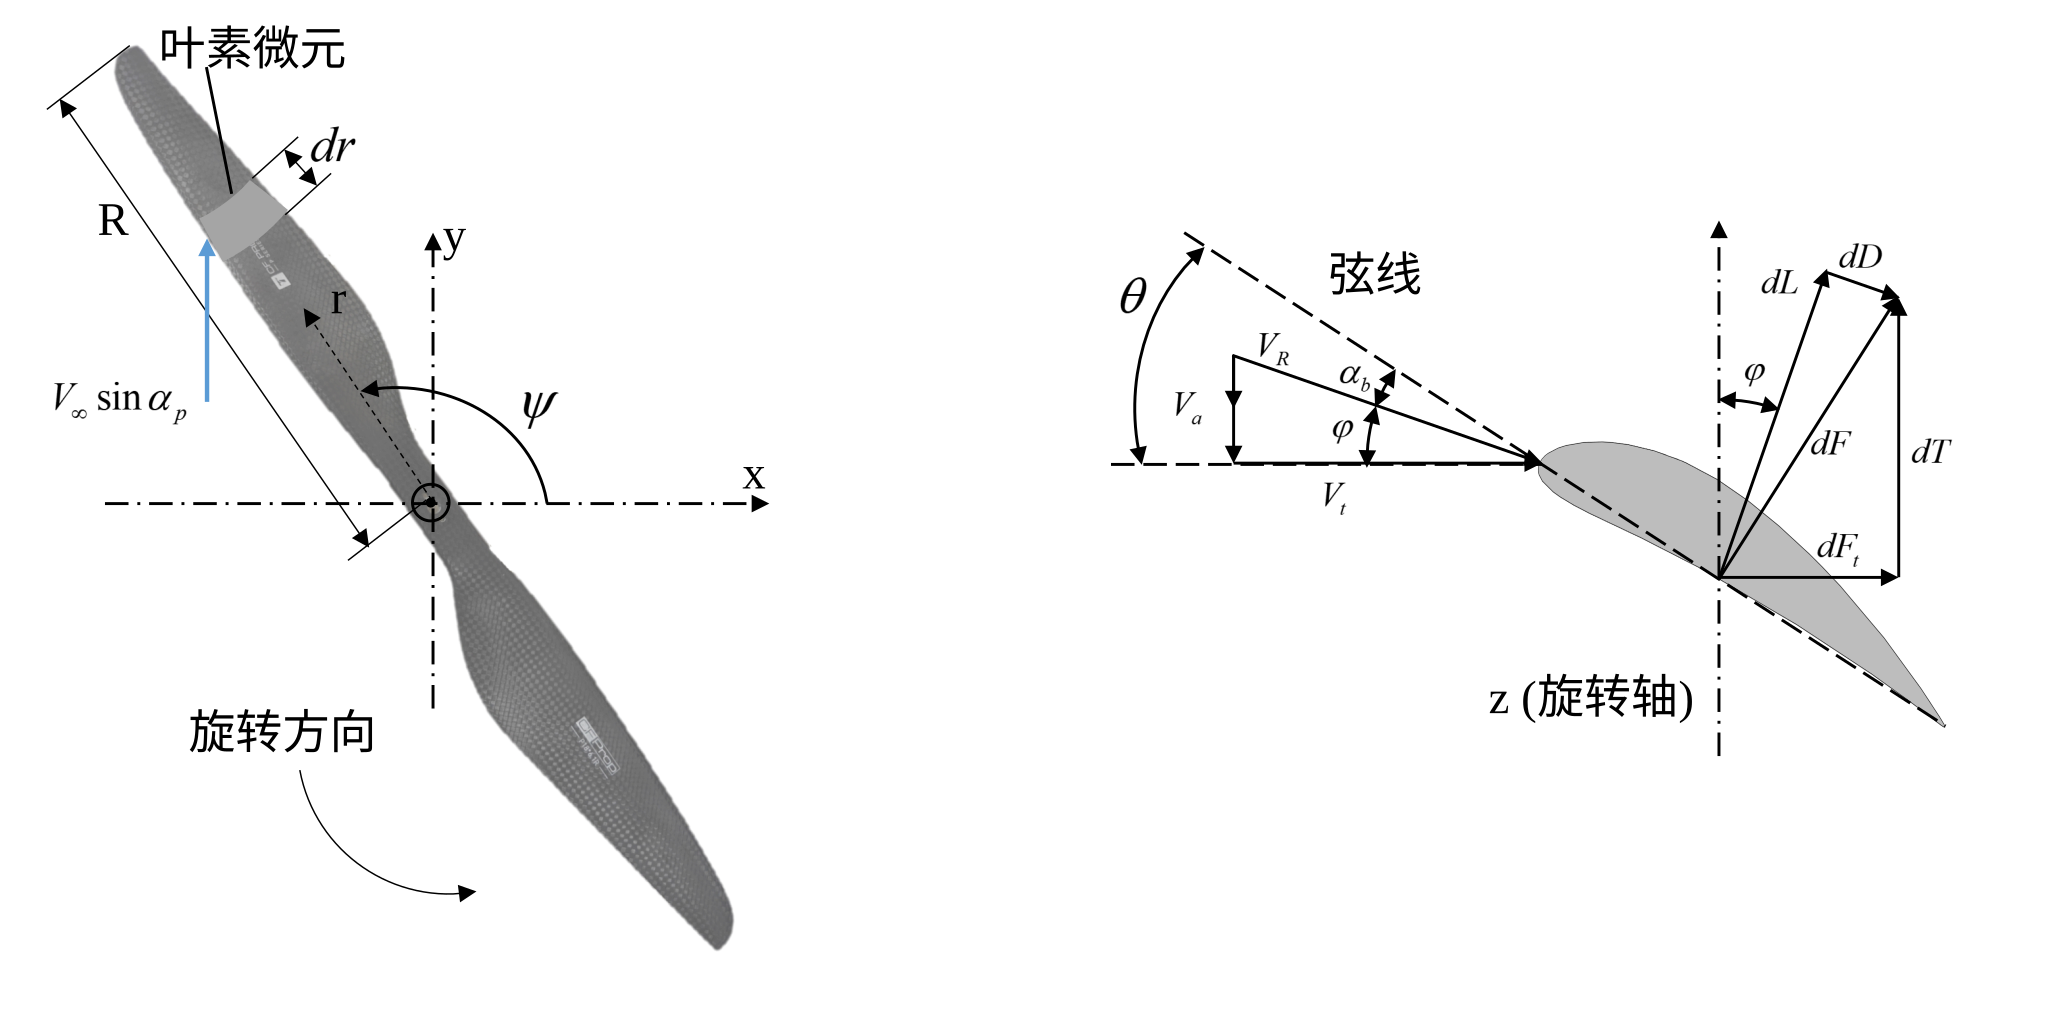
\includegraphics[width=6cm]{Image/fig2.pdf}}
\centerline{【图2：待插入图片】}
\vskip2mm
{\small 图2\quad 旋翼坐标、叶素离散及局部来流与气动力分解
\\
Fig.\,2\quad Rotor coordinates, blade element discretization and decomposition of local inflow and aerodynamic forces}}
\end{center}

\subsection{旋翼运动状态的定义}
\label{subsec:state_def}

综上, 当无人机运动时, 任一旋翼的运动状态可定义为与整机状态同构的五元组

\begin{equation}
\bm{s}_i=\left\{\bm{p}_i,\ \bm{v}_i,\ \bm{n}_i,\ \Omega_i,\ \psi_i\right\}
\label{eq:state_full}
\end{equation}

即桨毂位置、桨毂速度、桨盘姿态、旋翼转速与桨叶方位角. 由
式~(\ref{eq:hub_p})$\sim$式~(\ref{eq:psi_int}) 可知, $\bm{s}_i$ 完全由整机状态
$(\bm{p},\bm{v},\bm{q},\bm{\omega})$ 与安装参数 $(\bm{r}_i,\bm{n}_i,\sigma_i)$ 及转速 $\Omega_i$ 确定.
就气动建模而言, 影响轴向升力的不可约变量集合可进一步归约为

\begin{equation}
\bm{s}_i^{\mathrm{aero}}=\left\{V_{a,i},\ V_{\parallel,i},\ \psi_{w,i},\ \bm{\omega}_{\parallel},\ \Omega_i\right\}
\ \Longleftrightarrow\
\left\{\mu_i,\ \alpha_i,\ \psi_{w,i},\ \hat{\bm{\omega}}_{\parallel},\ Re_{\mathrm{tip}}\right\}
\label{eq:state_aero}
\end{equation}

于是旋翼轴向升力可紧凑地表示为 $T_i=f\!\left(\bm{s}_i^{\mathrm{aero}}\right)$,
其函数关系由第~\ref{subsec:lift}~节的叶素模型给出.
式~(\ref{eq:state_aero}) 表明, 复现高机动工况下的旋翼气动环境, 只需在地面同时给定
面内来流速度、来流倾角与桨盘所受过载三者. 本文所设计的旋转测试台正是通过悬臂长度、
悬臂转速与桨轴安装倾角三个自由度分别复现 $\left\{|\bm{a}_i|,\ V_{\parallel,i},\ \alpha_i\right\}$,
从而在式~(\ref{eq:state_aero}) 的意义下与飞行工况等价.

% ============================================================
% 符号表
% ============================================================
\begin{table}[htbp]
\centering
\caption{主要符号说明}
\label{tab:nomenclature}
\begin{tabular}{ll}
\toprule
符号 & 含义 \\
\midrule
$\mathcal{B},\ \mathcal{I}$ & 机体坐标系(前--右--下)、惯性坐标系(北--东--地) \\
$\bm{R}(\bm{q})$ & 由 $\mathcal{B}$ 至 $\mathcal{I}$ 的旋转矩阵 \\
$\bm{p},\ \bm{v},\ \bm{a}$ & 机体质心的位置、速度与加速度(惯性系) \\
$\bm{q},\ \bm{\omega}$ & 姿态四元数、机体角速度(机体系) \\
$\bm{v}_w$ & 环境风速(惯性系) \\
$\bm{r}_i,\ \bm{n}_i$ & 第 $i$ 个旋翼的安装位置与桨盘法向单位矢量(机体系) \\
$\sigma_i,\ \Omega_i,\ \psi_i$ & 旋翼转向符号、转速与桨叶方位角 \\
$\bm{p}_i,\ \bm{v}_i,\ \bm{a}_i$ & 桨毂中心的位置、速度与加速度 \\
$\bm{u}_i,\ \bm{u}_{\parallel,i}$ & 桨毂相对气流速度及其桨盘面内分量 \\
$V_{a,i},\ V_{\parallel,i}$ & 轴向来流速度、面内来流速度 \\
$\alpha_i,\ \psi_{w,i}$ & 来流倾角、来流方位角 \\
$\mu_i,\ \lambda_{c,i},\ \lambda_{\mathrm{ind},i}$ & 前进比、轴向入流比、诱导入流比 \\
$\chi_i$ & 尾迹偏斜角 \\
$\Omega_{e,i},\ \bm{\omega}_{\parallel}$ & 有效转速、机体角速度的桨盘面内分量 \\
$\rho,\ \psi$ & 叶素的展向位置与方位角 \\
$U_T,\ U_P,\ V_R$ & 叶素处的切向、法向相对速度与局部合速度 \\
$v_{\mathrm{ind}},\ k_x$ & 诱导速度、纵向入流梯度系数 \\
$\phi,\ \alpha_{\mathrm{eff}},\ \theta(\rho)$ & 入流角、有效迎角、几何扭转角 \\
$c(\rho),\ N_b,\ R_p,\ \rho_0$ & 弦长分布、桨叶片数、桨半径、桨根半径 \\
$C_l,\ C_d,\ C_T$ & 翼型升力系数、阻力系数、旋翼拉力系数 \\
$\rho_\infty,\ \mu_\infty$ & 空气密度、空气动力粘度 \\
$J_r,\ \bm{\tau}_{g,i}$ & 旋翼绕自转轴的转动惯量、陀螺力矩 \\
$n_i$ & 等效载荷因数 \\
$\Omega_a,\ R_0,\ \alpha_p$ & 转台角速度、旋翼中心到转台中心的距离、桨盘攻角 \\
\bottomrule
\end{tabular}
\end{table}

\section{控制架构}
\label{sec:control}

\subsection{传统控制架构及其局限性}
\label{subsec:conventional}

典型多旋翼飞控由位置-速度外环、姿态-角速度内环和控制分配器组成。外环根据位置与速度误差生成期望总推力和期望姿态，内环生成三轴期望力矩；控制分配器进一步将期望总推力与力矩分解为各旋翼的目标推力$f_{d,i}$。随后，推力-控制量映射器把$f_{d,i}$转换为归一化电机指令$u_i$，再由电子调速器、电机和螺旋桨产生实际推力$T_i$。该结构如图3所示。

在PX4等开源飞控中，目标推力通常通过含一次项和二次项的静态函数映射为归一化控制量，其一般形式为：
\begin{equation}
f_{d,i}=f_d(u_i)=c_a u_i^2+(1-c_a)u_i
\label{eq:static_map}
\end{equation}
式中，$c_a\in[0,1]$为表征推力曲线非线性的常参数。该式实质上利用固定系数近似旋翼推力随控制量或转速平方变化的关系，未显式考虑轴向来流、盘内来流、桨盘攻角和推进系统状态。

在近悬停、弱风和缓慢姿态变化条件下，式~(\ref{eq:static_map})能够满足常规控制需求；当局部来流发生显著变化时，相同$u_i$对应的$T_i$将随工况改变，导致$f_{d,i}$与$T_i$之间产生系统性偏差。由于传统架构缺少旋翼推力反馈，该偏差只能通过外层姿态或位置误差间接修正，控制作用链路较长，并可能在强扰动或快速机动时引起超调和振荡。

\begin{center}
\vbox{
%\centerline{\includegraphics[width=6cm]{Image/fig3.pdf}}
\centerline{【图3：待插入图片】}
\vskip2mm
{\small 图3\quad 传统多旋翼控制架构及旋翼推力开环映射
\\
Fig.\,3\quad Conventional multirotor control architecture and open-loop rotor thrust mapping}}
\end{center}

\subsection{升力闭环控制架构}
\label{subsec:closed_loop}

为使控制系统直接感知执行器层面的实际作用力，本文在控制分配器之后增加独立的旋翼升力内环。对第$i$个旋翼，目标推力$T_{c,i}$首先通过斜来流模型的逆映射生成前馈转速$\Omega_{ff,i}$；实际轴向推力$T_{m,i}$由同轴力传感器测量，反馈控制器根据误差$e_{T,i}=T_{c,i}-T_{m,i}$生成修正量$\Omega_{fb,i}$。最终转速指令为$\Omega_{c,i}=\Omega_{ff,i}+\Omega_{fb,i}$。该结构保持原有位置、姿态与控制分配逻辑不变，仅替换分配器之后的执行器映射，如图4所示。

\begin{center}
\vbox{
%\centerline{\includegraphics[width=8cm]{Image/fig4.pdf}}
\centerline{【图4：待插入图片】}
\vskip2mm
{\small 图4\quad 基于模型前馈与直接升力反馈的旋翼升力闭环控制架构
\\
Fig.\,4\quad Rotor lift closed-loop control architecture with model feedforward and direct lift feedback}}
\end{center}

\subsubsection{模型前馈与逆映射}
模型前馈决定了闭环在目标变化和工况切换时的基准控制量。Gonzalez-Morgado等采用静态二次模型生成PWM前馈，并利用力反馈补偿地面效应和天花板效应[12]；Liu等则依据风洞辨识的高保真推进模型，在当前工作点计算局部雅可比矩阵并用于增量动态逆控制[11]。前者结构通用，但在大范围斜来流下前馈失配较大；后者能够提高整机大机动条件下的分配精度，但依赖特定推进系统的全包线试验辨识和实时转速反馈。

本文从桨叶几何、翼型极线和局部速度分解出发建立叶素机理模型(第1节)。该高分辨率模型主要用于离线解释``局部速度---入流角---有效迎角---翼型气动力---轴向推力''的变化链条，并约束控制导向模型的输入变量和函数结构；在线控制不直接迭代求解完整叶素模型。完整叶素模型包含径向-方位二维积分、极线插值和诱导入流迭代，若直接部署于飞控内环，会增加计算量并引入数值收敛风险。为此，本文以旋翼转速$\Omega$、转台角速度$\Omega_a$和桨盘攻角$\alpha_p$为主要输入、轴向推力$T$为输出，在试验覆盖范围内离线生成高分辨率理论数据，并利用旋转测试台测量结果对系统残差进行校核，从而形成控制导向的简化模型$f_c(\Omega,\Omega_a,\alpha_p)$。该模型不追求复现全部局部流场，而是在叶素理论约束下选取低阶多项式或分段查表结构；其中，理论模型确定变量、单调性与主要交叉项，实验数据用于修正桨叶几何误差、二维极线误差和未建模诱导效应。该处理区别于完全由推力试验辨识的黑箱高保真模型，也避免将高维叶素求解直接置于在线控制回路。

对给定$T_c$、$\Omega_a$和$\alpha_p$，在可行转速区间内对$f_c$求逆，得到前馈转速$\Omega_{ff}=g(T_c,\Omega_a,\alpha_p)$。若采用查表实现，则以$T_c$、$\Omega_a$和$\alpha_p$为索引进行多维插值；若采用低阶显式模型，则选取满足单调性的实根，并施加最小、最大转速约束。

\subsubsection{直接推力反馈与传感器集成}
直接推力反馈要求传感器能够在不改变主要传力路径的条件下测量旋翼轴向作用力。应变片机臂测力方案易受结构模态、温漂与装配差异影响，而专用力传感器能够提供更直接的载荷观测[12,15]。本文采用小型拉压力传感器，并使其测量轴与电机轴线重合，以减少弯矩和横向载荷对轴向推力测量的耦合。

测量组件自上而下依次由螺旋桨、电机、上连接板、拉压力传感器和下连接板组成。螺旋桨产生的轴向推力经电机与上连接板传递至传感器受力端，再由下连接板传至机臂。传感器信号经零偏校准、比例换算和低通滤波后得到$T_m$。对于旋转测试台，还需通过静止和空载旋转试验评估离心载荷、结构振动及线缆牵引对测量通道的影响。

\subsubsection{力感知飞控架构}
推力内环位于控制分配器与电机输出模块之间，其更新频率高于外层姿态和位置回路。PX4中的控制分配器仍输出各旋翼归一化目标推力[16]，新增模块将其换算为物理目标推力$T_c$，并计算$\Omega_{ff}$与$\Omega_{fb}$；修正后的电机指令送入原有电机输出链路。通过在旋翼力层面闭环，执行器扰动可在显著影响机体姿态之前被检测和修正。为避免积分饱和，反馈项设置幅值与积分限幅，并在未检测到有效推力、传感器异常或电机停转时退出闭环。

最终控制指令由模型前馈与直接推力反馈叠加：
\end{multicols}%开始通栏显示
\begin{equation}
\Omega_c=\Omega_{ff}+\Omega_{fb}=g(T_c,\Omega_a,\alpha_p)+C_{fb}(T_c-T_m)
\label{eq:control_law}
\end{equation}
\begin{multicols}{2}%开始双栏显示
式中，$C_{fb}$表示推力反馈控制器，可采用带积分限幅的PID或其他稳定补偿器。模型前馈承担主要稳态控制量，直接力反馈用于抑制模型残差、动态入流、螺旋桨个体差异及外部扰动。

\section{实验}
\label{sec:experiment}

为验证所提出的旋翼升力模型与升力闭环控制器，本文在旋转测试台上开展两类实验：其一，执行如表1所示的全包线工况测试，将第1节机理模型的预测升力与实测升力对比，验证模型精度；其二，在气动效应最显著、来流垂直于桨盘平面的90$^{\circ}$攻角工况下，模拟两个场景——场景1缓慢加速，模拟稳态来流作用下的影响；场景2以最大加速度运行，模拟机动飞行时的动态来流影响，并分别按表2所示的5组方案验证闭环控制效果。

\subsection{桨叶几何与翼型气动数据获取}
\label{subsec:geo}

以T-Motor P18$\times$6.1\,CF螺旋桨为对象，采用摄影测量技术建立桨叶三维模型。拍摄时使桨叶表面具有充分纹理，并从不同方位和俯仰角获取重叠图像；利用RealityScan完成特征匹配、稠密点云重建和网格生成，再将模型坐标系的$z$轴与旋转轴对齐。

在给定$r/R$位置处以圆柱面与桨叶网格求交，将截面点投影至局部二维坐标系，并对上、下表面进行平滑拟合。由拟合截面得到弦长$c(\rho)$、安装角$\theta(\rho)$和相对厚度$t/c$；归一化后的截面坐标用于翼型极线计算。摄影测量与截面提取过程如图5所示。

\begin{center}
\vbox{
%\centerline{\includegraphics[width=6cm]{Image/fig5.pdf}}
\centerline{【图5：待插入图片】}
\vskip2mm
{\small 图5\quad 螺旋桨摄影测量、三维重建与截面提取过程
\\
Fig.\,5\quad Photogrammetry, 3D reconstruction and cross-section extraction of the propeller}}
\end{center}

沿$0.15R$-$0.95R$范围选取10个代表性截面，获得弦长、安装角和相对厚度的径向分布。为检验几何提取可靠性，将提取结果与公开的同尺度桨叶几何或手工测量结果进行对比，并统计弦长与安装角误差。

\begin{center}
\vbox{
%\centerline{\includegraphics[width=6cm]{Image/fig6.pdf}}
\centerline{【图6：待插入图片】}
\vskip2mm
{\small 图6\quad 桨叶截面拟合及弦长、安装角的径向分布
\\
Fig.\,6\quad Blade section fitting and radial distribution of chord and pitch angle}}
\end{center}

针对提取的各径向截面，利用XFOIL计算不同有效迎角$\alpha_{\mathrm{eff}}$与雷诺数$Re$下的二维翼型气动系数[13]，建立供第~\ref{subsec:lift}~节叶素模型查取的极线表$C_l(\alpha_{\mathrm{eff}},Re)$、$C_d(\alpha_{\mathrm{eff}},Re)$。计算中将极线统一整理至$-10^{\circ}\le\alpha_{\mathrm{eff}}\le40^{\circ}$及离散$Re$网格。对个别截面在高迎角或低雷诺数下未收敛的点，先采用相邻工况插值；超出查表范围时采用边界截断，以避免外推导致的非物理解。该处理保证模型数值稳定，但大迎角失速区的二维极线误差仍需由实验校核。

\subsection{高机动工况构造：旋翼测试台}
\label{subsec:bench}

为在地面条件下构造可重复的斜来流工况，本文搭建旋转悬臂式单旋翼测试平台，如图7所示。驱动电机带动转盘和悬臂绕竖直轴旋转，旋翼推进单元安装于半径$R_0$处；通过倾转支架调节桨盘攻角$\alpha_p$，通过转台角速度$\Omega_a$改变旋翼中心的相对来流速度。平台悬臂长度为1.5\,m，最高角速度约6.8\,rad/s，对应末端线速度约10.2\,m/s。

\begin{center}
\vbox{
%\centerline{\includegraphics[width=8cm]{Image/fig7.pdf}}
\centerline{【图7：待插入图片】}
\vskip2mm
{\small 图7\quad 旋转测试台实物、旋翼安装方式与主要几何参数
\\
Fig.\,7\quad Rotating test bench, rotor mounting and main geometric parameters}}
\end{center}

与风洞试验将旋翼中心来流近似为均匀自由流不同，旋转测试台由悬臂回转生成相对来流。由于桨盘内不同叶素到转台中心的瞬时距离不同，局部来流速度随展向位置$\rho$和方位角$\psi$变化；当$\alpha_p\neq0$时，该来流同时具有垂直于桨盘的轴向分量和位于桨盘内的切向分量，形成方位非均匀入流。设转台角速度为$\Omega_a$、旋翼中心到转台中心的距离为$R_0$、旋翼角速度为$\Omega$，对位于$(\rho,\psi)$处的叶素，局部轴向速度$V_a$和盘内切向速度$V_t$表示为：
\end{multicols}%开始通栏显示
\begin{equation}
\begin{aligned}
V_a(\rho,\psi)&=\Omega_a(R_0-\rho\cos\psi)\sin\alpha_p+v_i\\
V_t(\rho,\psi)&=\Omega\rho-\Omega_a(R_0-\rho\cos\psi)\cos\alpha_p\cos\psi
\end{aligned}
\label{eq:bench_vel}
\end{equation}
\begin{multicols}{2}%开始双栏显示
式中，$v_i$为诱导速度。由局部速度分量可得入流角$\varphi=\arctan(V_a/V_t)$，叶素有效迎角为$\alpha_b=\theta(\rho)-\varphi$。由式~(\ref{eq:bench_vel})可知，转台角速度$\Omega_a$与桨盘攻角$\alpha_p$通过改变$V_a$和$V_t$，进一步改变入流角、有效迎角及叶素气动力分布。因此，相同旋翼转速在不同斜来流工况下对应不同轴向推力，这正是静态推力映射失准的机理来源。

需要说明的是，测试台通过桨盘攻角$\alpha_p$与第~\ref{subsec:inflow}~节的来流倾角$\alpha_i$对应，通过末端线速度$\Omega_a R_0$与面内来流$V_{\parallel,i}$对应，即
\begin{equation}
V_{\parallel,i}=\Omega_a R_0\cos\alpha_p,\qquad
V_{a,i}=\Omega_a R_0\sin\alpha_p
\label{eq:bench_map}
\end{equation}
代入式~(\ref{eq:mu_lambda})即可得到测试台工况下的前进比$\mu_i$与轴向入流比$\lambda_{c,i}$，进而由式~(\ref{eq:glauert})确定平均诱导入流比$\lambda_{\mathrm{ind},i}$。与飞行工况的区别在于，测试台悬臂长度$R_0$与桨盘半径$R_p$量级相当，故还需在叶素速度场中显式保留式~(\ref{eq:bench_vel})的径向非均匀项，即将第~\ref{subsec:blade_element}~节中均匀的$V_{a,i}$、$V_{\parallel,i}$替换为随$(\rho,\psi)$变化的局部值。该径向非均匀项正是旋转测试台区别于风洞均匀来流、能够更真实复现高机动斜来流的关键。

在实际测试中，0-10\,m/s左右的来流下，转速-控制量之间的关系基本恒定，影响升力的是实际升力-实际转速之间的关系。为使前馈项的转速输出能够发挥作用，需要先标定转速-控制量之间的静态映射关系：在固定台架上选择0-100\%油门之间的13个固定点位，读取对应的电机控制量和实际转速，拟合得到
\begin{equation}
u_{ff}=a\omega^2+b\omega+c
\label{eq:rpm_calib}
\end{equation}
其中，$a,b,c$为拟合出的常系数。该式还会随着电池压降发生变化，但是这种扰动能够被力反馈补偿，因此该式只需给出相对正确的转速-控制量关系即可。

旋翼测试台基本参数如表3所示，根据$\tau=J\dot{\omega}$，带负载能达到的最大角加速度为7.38\,rad/s$^{2}$，从零加速到最大转速所需的最小时间为0.92\,s。设置从0-100\%转速的时间为1\,s，模拟高机动飞行时无人机的加速过程，构造动态来流。

\begin{center}
\vbox{\centering{\small 表3\quad 参数定义
\\
Table\,3 \quad Parameter definitions} \vskip2mm
{\footnotesize\centering
\begin{tabular}{cc}
\toprule
参数 & 值 \\
\midrule
$k_p$ & 0.025 \\
$k_i$ & 0.05 \\
$a$ & $2.6972\times10^{-8}$ \\
$b$ & $1.829\times10^{-5}$ \\
$c$ & $3.718\times10^{-2}$ \\
总转动惯量 $I$ & 9.42\,kg$\cdot$m$^{2}$ \\
悬臂长度 & 1.5\,m \\
最大转速 & 63\,rpm \\
最大扭矩 & 69.5\,N$\cdot$m \\
\bottomrule
\end{tabular}}}
\end{center}

测试对象为T-Motor MN5008 KV340电机与P18$\times$6.1\,CF螺旋桨，旋翼轴向推力由同轴拉压力传感器测量，转台角度与角速度由编码器/飞控惯性测量单元记录，电机转速由独立转速测量通道获取。试验选取约3000、4000和5000\,r/min的典型转速，桨盘攻角覆盖0$^{\circ}$-90$^{\circ}$(间隔15$^{\circ}$)，并在不同$\Omega_a$下改变旋翼中心来流速度，构成表1所示的全包线工况矩阵。每个工况在转台与旋翼转速稳定后采集数据，剔除启动和制动阶段，再计算稳态均值、标准差与频域特征。

\begin{center}
\vbox{\centering{\small 表1\quad 旋翼测试台测试设置
\\
Table\,1 \quad Test settings of the rotor test bench} \vskip2mm
{\footnotesize\centering
\begin{tabular}{ccc}
\toprule
转速档位 & 攻角 & 来流速度 \\
\midrule
3000\,rpm & \multirow{3}{*}{0-90$^{\circ}$(间隔15$^{\circ}$)} & \multirow{3}{*}{0-10.2\,m/s(间隔10\%)} \\
4000\,rpm & & \\
5000\,rpm & & \\
\bottomrule
\end{tabular}}}
\end{center}

【待补充表1备注：转台半径、$\Omega_a$分档、实际转速均值、$\alpha_p$分档、采样频率、单工况持续时间及重复次数；同时说明推力传感器量程、标定误差和滤波带宽。】

\subsection{旋翼升力模型精度验证}
\label{subsec:model_verif}

由于测试过程中实际电机转速、来流不可避免会发生波动，因此引入前进比来统一反映旋翼面对的来流，定义为：
\begin{equation}
J=\frac{V_\infty}{nD}
\label{eq:advance}
\end{equation}
其中$V_\infty$是来流速度，$n$为旋翼转速(单位rps)，$D$为旋翼桨盘直径。

模型精度的衡量指标为升力系数$C_T$，定义为：
\begin{equation}
C_T=\frac{T}{\rho n^2 D^4}
\label{eq:CT}
\end{equation}
其中，$T$为旋翼产生的轴向升力，$\rho$为空气密度。

【待补充图8及定量结果：不同转速、攻角与来流速度下机理模型预测的$C_T$与实测值的对比，报告模型MAE/MAPE及误差随$\mu$、$\alpha_p$的分布，说明机理模型在斜来流工况下的精度及其残差来源。】

\subsection{升力闭环控制效果验证}
\label{subsec:control_verif}

控制实验设置如表2所示的5组对比方案，覆盖静态二次映射、斜来流逆模型前馈与直接推力反馈的不同组合。

\begin{center}
\vbox{\centering{\small 表2\quad 控制方法验证方案
\\
Table\,2 \quad Verification schemes of the control method} \vskip2mm
{\footnotesize\centering
\begin{tabular}{ccc}
\toprule
方案 & 前馈 & 反馈 \\
\midrule
1 & 静态二次模型 & 关闭 \\
2 & 旋翼模型前馈 & 关闭 \\
3 & 关闭 & 开启 \\
4 & 静态二次模型 & 开启 \\
5 & 旋翼模型前馈 & 开启 \\
\bottomrule
\end{tabular}}}
\end{center}

通过阶跃目标推力、转台加速/减速和桨盘攻角切换构造目标变化与外部扰动，评价上升时间、调节时间、稳态误差、峰值误差和RMSE。所有方案保持相同的外层控制指令、限幅和数据处理流程。

【待补充图9-图10及定量结果：各方案的$T_c$、$T_m$、$\Omega_c$和$e_T$时序；报告闭环相对开环的RMSE与峰值误差降低幅度，并给出统计显著性或重复试验离散性。】

\section{结论}

本文面向低空经济应用中多旋翼无人机在复杂气流和快速机动条件下的推进系统推力失配问题，建立了从整机运动状态到单旋翼轴向升力的机理模型，并提出基于模型前馈与直接力反馈的升力闭环控制方法。首先，通过坐标系定义、桨毂运动学与相对来流分解，将旋翼气动状态归约为轴向与面内来流、来流方位角、桨盘面内角速度与转速所构成的低维集合；在此基础上，结合摄影测量桨叶几何、XFOIL翼型极线和考虑诱导速度非均匀分布的叶素理论，建立了可解释的旋翼升力模型。其次，分析了传统开环推力映射在高机动斜来流下的失配机理，并在控制分配器之后引入直接升力内环，使模型前馈提供主要控制量、力反馈补偿模型残差与外部扰动。最后，搭建了桨盘攻角与转台角速度可调的旋转测试平台，构造了具有方位非均匀特征的斜来流入流，并对升力模型精度与闭环控制效果进行了验证。

实验结果显示，【待补充：模型误差与闭环性能的核心定量结论】。现阶段结论适用于所测试的单旋翼、转速和桨盘攻角范围。

本文方法在模型与反馈之间进行了功能分工：叶素模型提供物理可解释的变量与结构约束，控制导向逆模型提供主要前馈量，直接力反馈补偿剩余误差。与全包线风洞辨识模型相比，该方法减少了对专用风洞和大规模推进系统标定的依赖，但其精度仍受摄影测量几何误差、二维翼型极线、大迎角失速和准稳态假设影响。与仅采用二次模型前馈的旋翼力控制相比，斜来流模型可降低反馈回路的基准补偿负担，但增加了$\Omega_a$和$\alpha_p$等工况量的获取或估计需求。当前验证仍局限于单旋翼旋转测试台，转台生成的是确定性周期来流，尚不能完全覆盖真实飞行中的动态入流、旋翼间干扰和机体尾流；旋转结构的向心载荷与振动也可能耦合到力传感器。未来将重点研究动态入流建模、旋转测试台惯性载荷补偿、工况量在线估计以及多旋翼整机飞行验证。

\section*{致谢}

【待填写：对研究工作和本文写作给予支持的组织或个人表示感谢；基金项目请标注在首页页脚。】

\begin{thebibliography}{99}
\zihao{6} \addtolength{\itemsep}{0.2em} \urlstyle{rm}

\bibitem{1} 中国科学院地理科学与资源研究所. 中国低空经济发展指数报告(2025)[EB/OL]. 2025-05-07

\bibitem{2} 陈林, 缪志强, 王祥科, 等. 自主飞行器技术及其在低空经济中的应用综述[J]. 机器人, 2025, 47(3): 470-496

\bibitem{3} 张军, 陈磊, 高智杰. 低空无人机技术研究现状与展望[J]. 中国工程科学, 2025, 27(2): 73-85

\bibitem{4} Brandt J B, Selig M S. Propeller performance data at low Reynolds numbers[C]//49th AIAA Aerospace Sciences Meeting. Orlando: AIAA, 2011: AIAA 2011-1255

\bibitem{5} Theys B, Dimitriadis G, Hendrick P, et al. Experimental and numerical study of micro-aerial-vehicle propeller performance in oblique flow. {\sl Journal of Aircraft}, 2017, {\bf 54}(3): 1076-1084

\bibitem{6} Serrano D, Ren M, Qureshi A J, et al. Effect of disk angle-of-attack on aerodynamic performance of small propellers. {\sl Aerospace Science and Technology}, 2019, {\bf 92}: 901-914

\bibitem{7} Simmons B M. System identification for propellers at high incidence angles. {\sl Journal of Aircraft}, 2021, {\bf 58}(6): 1336-1350

\bibitem{8} Itoh Y, Satoh A. Modeling and numerical investigation of aerodynamic characteristics of a propeller circling on a whirling arm. {\sl Transactions of the Japan Society for Aeronautical and Space Sciences}, 2021, {\bf 64}(6): 335-347

\bibitem{9} Gill R, D'Andrea R. Propeller thrust and drag in forward flight[C]//2017 IEEE Conference on Control Technology and Applications. IEEE, 2017: 73-79

\bibitem{10} Bauersfeld L, Kaufmann E, Foehn P, et al. NeuroBEM: Hybrid aerodynamic quadrotor model[C]//Robotics: Science and Systems XVII. 2021

\bibitem{11} Liu H, Lin D, Ye J, et al. Quadrotor aggressive control based on angular acceleration feedback and high-fidelity propulsion model. {\sl IEEE Transactions on Industrial Electronics}, 2025

\bibitem{12} Gonzalez-Morgado A, Sanchez-Cuevas P J, Heredia G, et al. Rotor-force controller for multirotors under aerodynamic interferences. {\sl Aerospace Science and Technology}, 2025, {\bf 157}: 109861

\bibitem{13} Drela M. XFOIL: An analysis and design system[M]//Low Reynolds Number Aerodynamics. Berlin: Springer, 1989: 1-12

\bibitem{14} Bangura M, Mahony R. Thrust control for multirotor aerial vehicles. {\sl IEEE Transactions on Robotics}, 2017, {\bf 33}(2): 390-405

\bibitem{15} Davis E, Pounds P E I. Direct sensing of thrust and velocity for a quadrotor rotor array. {\sl IEEE Robotics and Automation Letters}, 2017, {\bf 2}(3): 1360-1366

\bibitem{16} Meier L, Honegger D, Pollefeys M. PX4: A node-based multithreaded open source robotics framework for deeply embedded platforms[C]//2015 IEEE International Conference on Robotics and Automation. IEEE, 2015: 6235-6242

\bibitem{17} 蒋涵, 陈泽昊, 常彦春, 等. 基于直接升力控制的旋翼无人机风扰抑制方法[J]. 中国科学: 技术科学, 2026: 1-13

\bibitem{18} 蒋涵, 常彦春, 杨丽英, 等. 基于升力反馈的旋翼无人机控制方法[J]. 机器人, 2026, 48(3): 518-530

\end{thebibliography}

% TODO: 请作者填写作者简介(姓名、职称、学习工作经历、研究方向)与照片
\begin{biographynophoto}
\noindent{\hei 【待填写作者姓名】}\quad 【待填写作者简介】.\\E-mail: 【待填写邮箱】

\noindent({\bf 【待填写英文作者姓名】}\quad 【待填写英文作者简介】.)
\end{biographynophoto}

\end{multicols}
\end{document}
